\chapter{Hardware Development}

\section{Circuit Design \& Simulation}

\subsection{Electret Microphone Circuit}
First, tried to simulate the electrec microphone circuit using LTSpice. The circuit is shown in the figure below.

\begin{figure}[h]
	\centering
	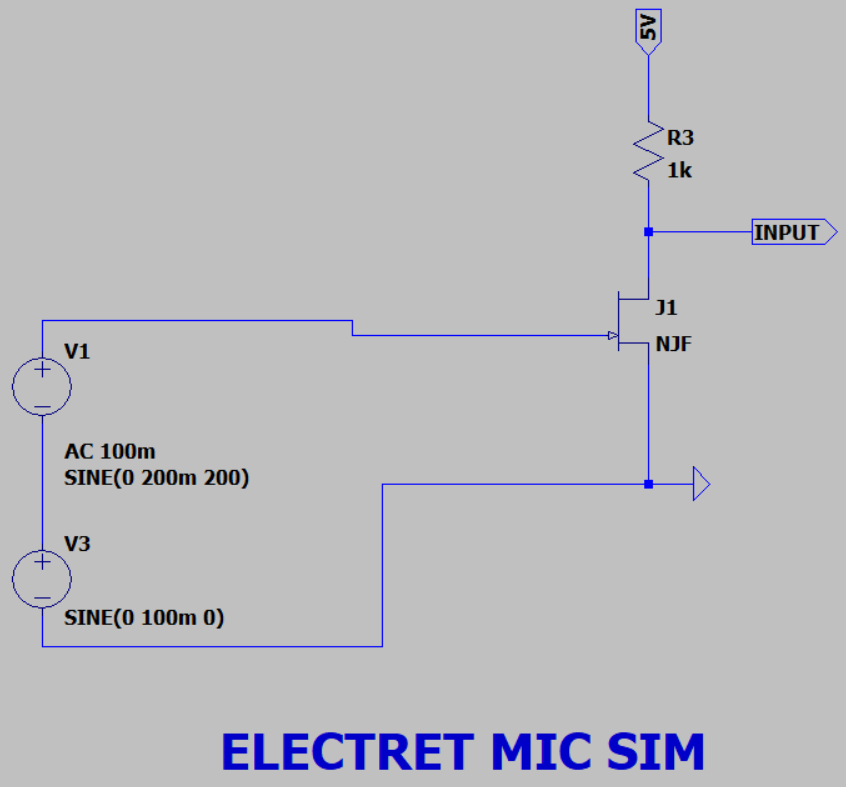
\includegraphics[width=0.6\textwidth]{assets/mic_circuit.png}
	\caption{Electret Microphone Circuit}
	\label{fig:mic_circuit}
\end{figure}

A 2-wire electrec microphone consists of one capacitor and one N-channel JFET. Using the circuit shown in Figure \ref{fig:mic_circuit}, we we able to acquire the voice signal from the microphone. Signal was too weak and too noisy to be used directly, so we needed to amplify and filter it.

\newpage
\thispagestyle{plain}

\subsection{Filter Circuit}

\subsubsection{High-Pass \& DC Filter}
Incoming signal was oscillating around 5V and had a lot of noise. We were planning to Arduino Uno for signal processing, so we needed to convert the signal to 0-5V range. We also needed to filter the noise. We designed a filter circuit using LTSpice.
\begin{figure}[h]
	\centering
	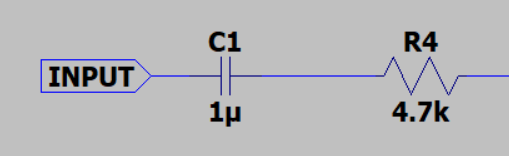
\includegraphics[width=0.6\textwidth]{assets/high-pass.png}
	\caption{High-Pass Filter Circuit}
	\label{fig:hp_filter_circuit}
\end{figure}

Used a passive high-pass filter setup as shown in Figure \ref{fig:hp_filter_circuit} for both filtering DC offset and low frequency noise. The cutoff frequency can be calculated using the formula:
\begin{equation}\label{eq:filter_cutoff}
	f_c = \frac{1}{2\pi RC}
\end{equation}
In our case, we used R = $4.7k\Omega$ and C = $1\mu$F, so the cutoff frequency was $33.8$Hz. This filter was able to filter out the DC offset and low frequency noise.

\subsubsection{Low-Pass Filter}

\begin{figure}[h]
	\centering
	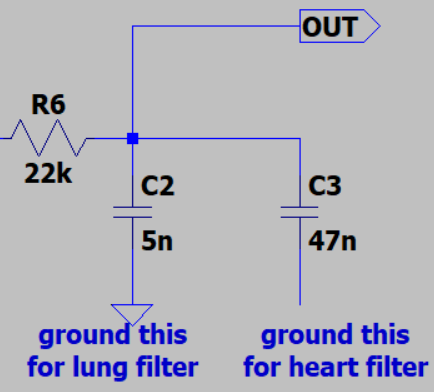
\includegraphics[width=0.5\textwidth]{assets/low-pass.png}
	\caption{Low-Pass Filter Circuit}
	\label{fig:lp_filter_circuit}
\end{figure}

Again, used a passive low-pass filter setup as shown in Figure \ref{fig:lp_filter_circuit} for filtering high frequency noise. The cutoff frequency can be calculated using the formula \ref{eq:filter_cutoff}. In our case, we used R = $22k\Omega$ and C = $5$nF for lung, C = $47$nF for heart, so the cutoff frequency was $153$Hz for heart and $1446$Hz for lung. This filter was able to filter out the high frequency noise.

\newpage
\thispagestyle{plain}

\subsection{Amplifier Circuit}

\begin{figure}[h]
	\centering
	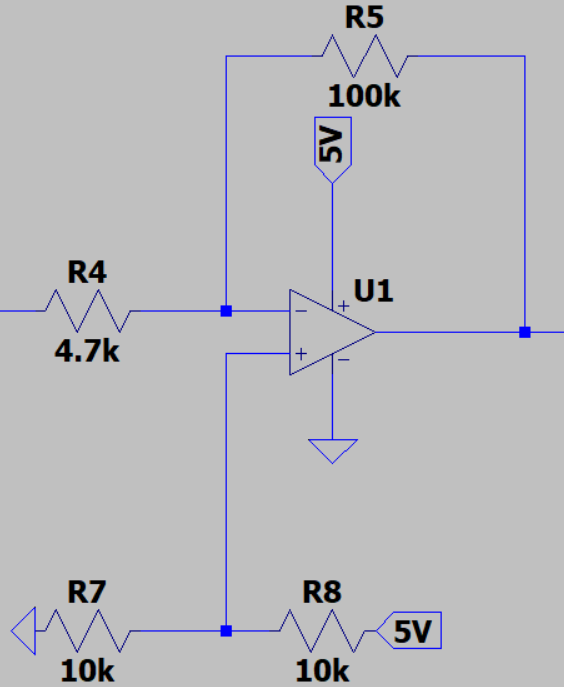
\includegraphics[width=0.6\textwidth]{assets/amplifier.png}
	\caption{Amplifier Circuit}
	\label{fig:amplifier_circuit}
\end{figure}

We used an inverting op-amp circuit for amplifying the signal, adding 2.5V DC bias, and inverting the signal to its original state (because the signal was inverted by the electrec mic). The gain of the amplifier can be calculated using the formula:

\begin{equation}\label{eq:amplifier_gain}
	G = -\frac{R_f}{R_1}
\end{equation}

In our case, we used $R_1 = 4.7k\Omega$ and $R_f = 100k\Omega$, so the gain was approximately $-20$. This amplifier was able to amplify the signal to a usable level. For DC bias, we used a voltage divider ciruit to get 2.5V and connected it to the non-inverting input of the op-amp, which made our signal oscillate around 2.5V.

\newpage
\thispagestyle{plain}

\subsection{Final Circuit}

After connecting everything together, the final circuit looked like this:

\begin{figure}[h]
	\centering
	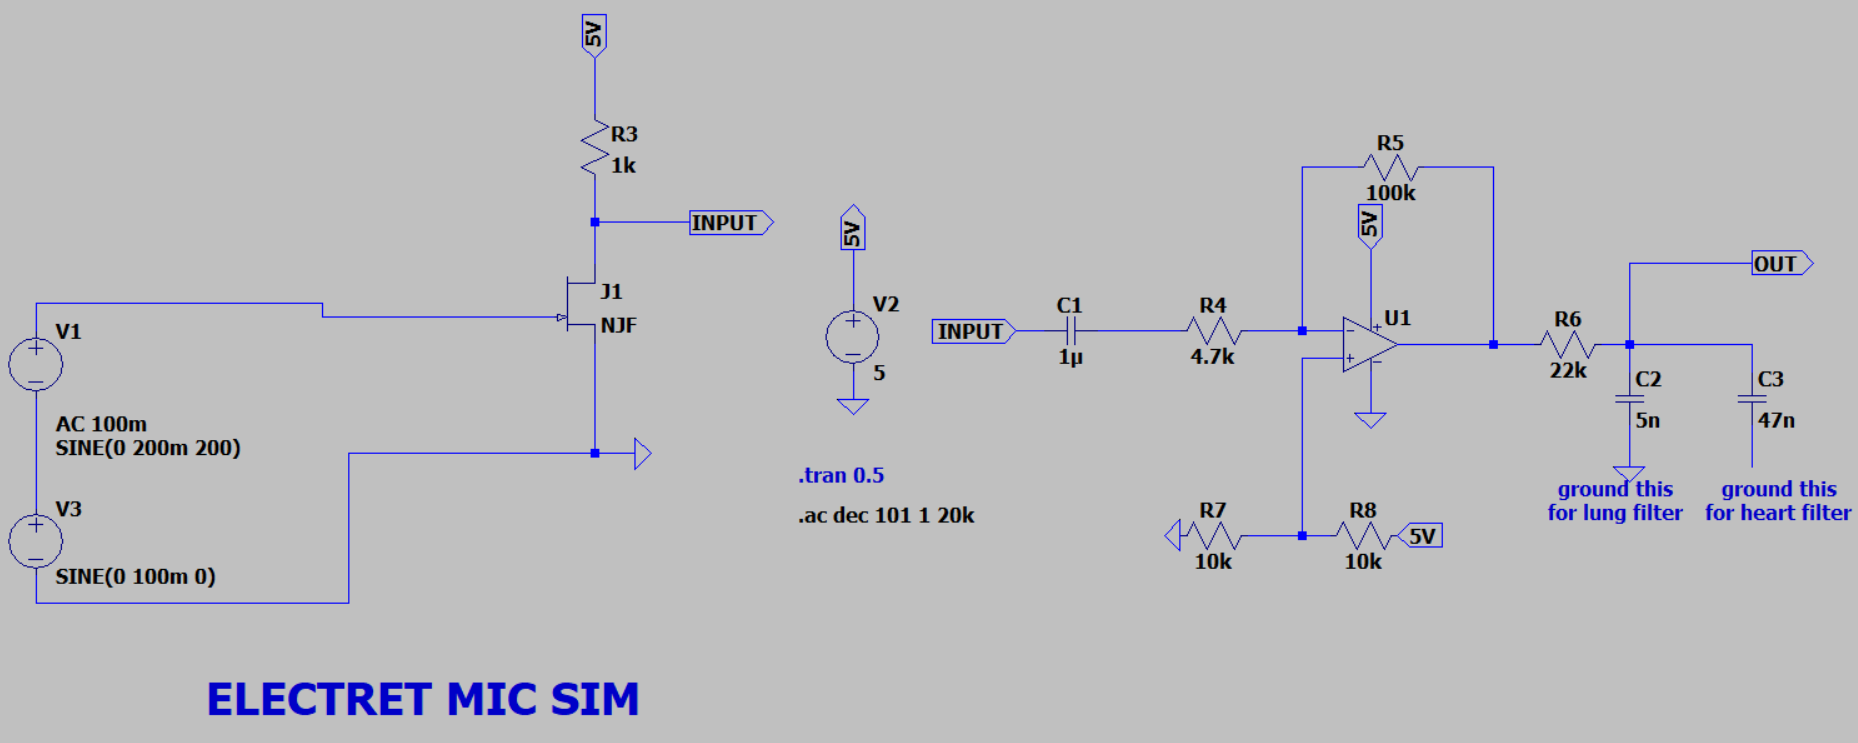
\includegraphics[width=1\textwidth]{assets/final-circuit.png}
	\caption{Final Circuit}
	\label{fig:final_circuit}
\end{figure}

To test the circuit, we used a function generator to simulate the electrec microphone signal. We were able to get the signal from the microphone, amplify it, and filter it successfully. After building the circuit we ran an AC simulation on LTSpice and checked the cutoff frequencies.

\begin{table}[h]
	\begin{tabular}{l|l|l|}
		\cline{2-3}
		                                                & \textbf{Analytical Cutoff Frequency} & \textbf{Simulation Result} \\ \hline
		\multicolumn{1}{|l|}{\textbf{High-Pass}}        & 33.8Hz                               & 26.7Hz                     \\ \hline
		\multicolumn{1}{|l|}{\textbf{Low-Pass (Heart)}} & 153Hz                                & 205Hz                      \\ \hline
		\multicolumn{1}{|l|}{\textbf{Low-Pass (Lung)}}  & 1466Hz                               & 1530Hz                     \\ \hline
	\end{tabular}
	\caption{Cutoff Frequencies}
	\label{tab:cutoff_frequencies}
\end{table}

According to \textcite{Debbal2020}, these frequencies are suitable for heartbeat detection and according to \textcite{Gross2000}, these frequencies are suitable for lung sound detection.

\newpage
\thispagestyle{plain}

\section{Prototype Design}

\subsection{Breadboard Prototype}
We have built the circuit in Figure \ref{fig:final_circuit} on a breadboard and measured output voltages using an oscilloscope.

\begin{figure}[h]
	\centering
	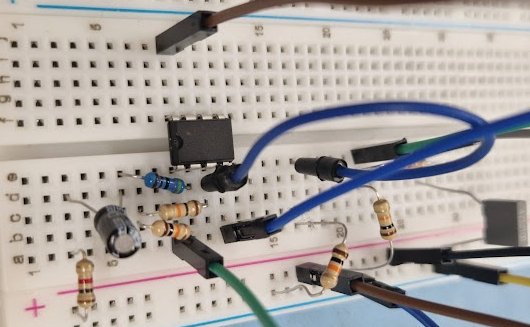
\includegraphics[width=0.7\textwidth]{assets/breadboard.png}
	\caption{Breadboard Prototype}
	\label{fig:breadboard_prototype}
\end{figure}

\begin{figure}[h]
	\centering
	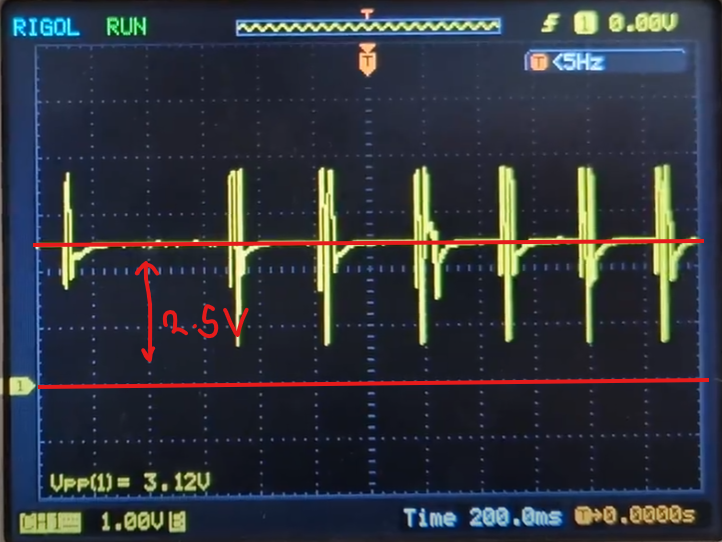
\includegraphics[width=0.5\textwidth]{assets/breadboard-output.png}
	\caption{Breadboard Prototype Output}
	\label{fig:breadboard_prototype_output}
\end{figure}

Output was exactly as expected. We were able to get the signal from the microphone, amplify it, give 2.5V DC bias, and filter it successfully.

\newpage
\thispagestyle{plain}

\subsection{Pertinax Board Design}

After making sure that the circuit works as expected, we soldered the circuit parts to perforated pertinax board as shown in Figure \ref{fig:pertinax_board_design}.

\begin{figure}[h]
	\centering
	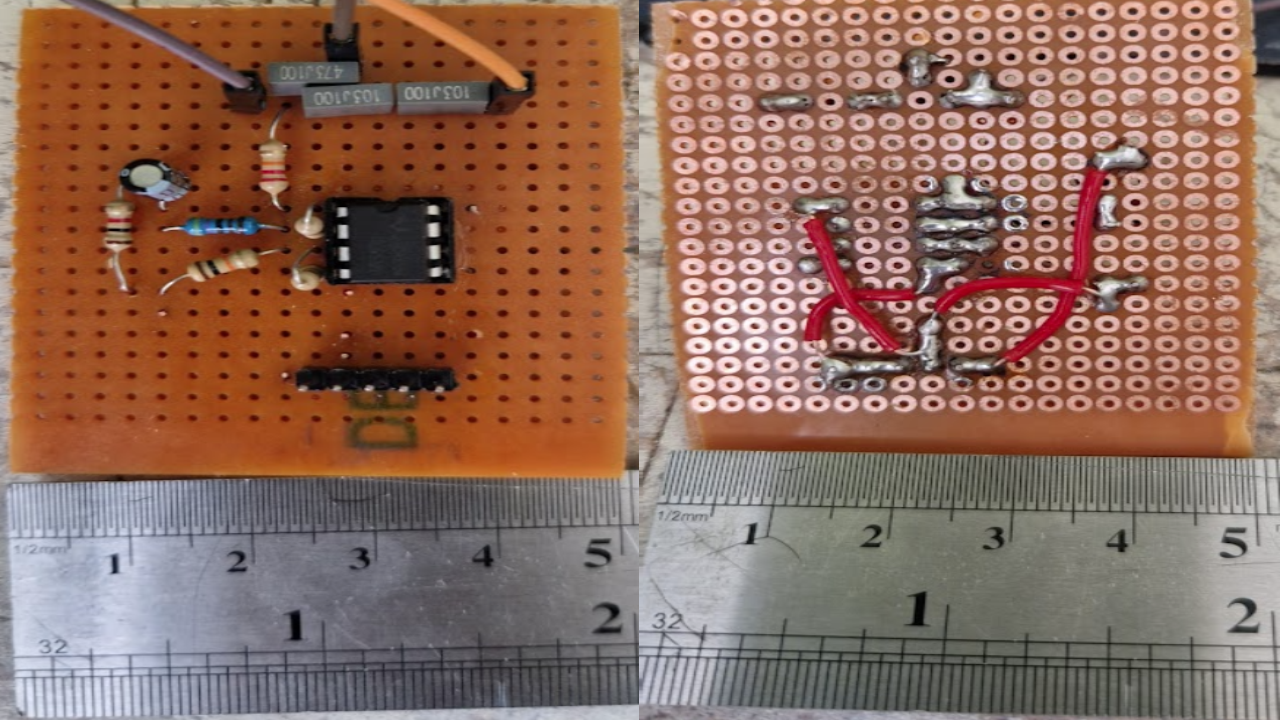
\includegraphics[width=1\textwidth]{assets/pertinax-design.png}
	\caption{Pertinax Board Design}
	\label{fig:pertinax_board_design}
\end{figure}

\newpage
\thispagestyle{plain}

\subsection{Casing Design}

We designed a casing for the prototype using SolidWorks. Casing has required pin headers for microphone, Arduino, and power supply connections.

\begin{figure}[h]
	\centering
	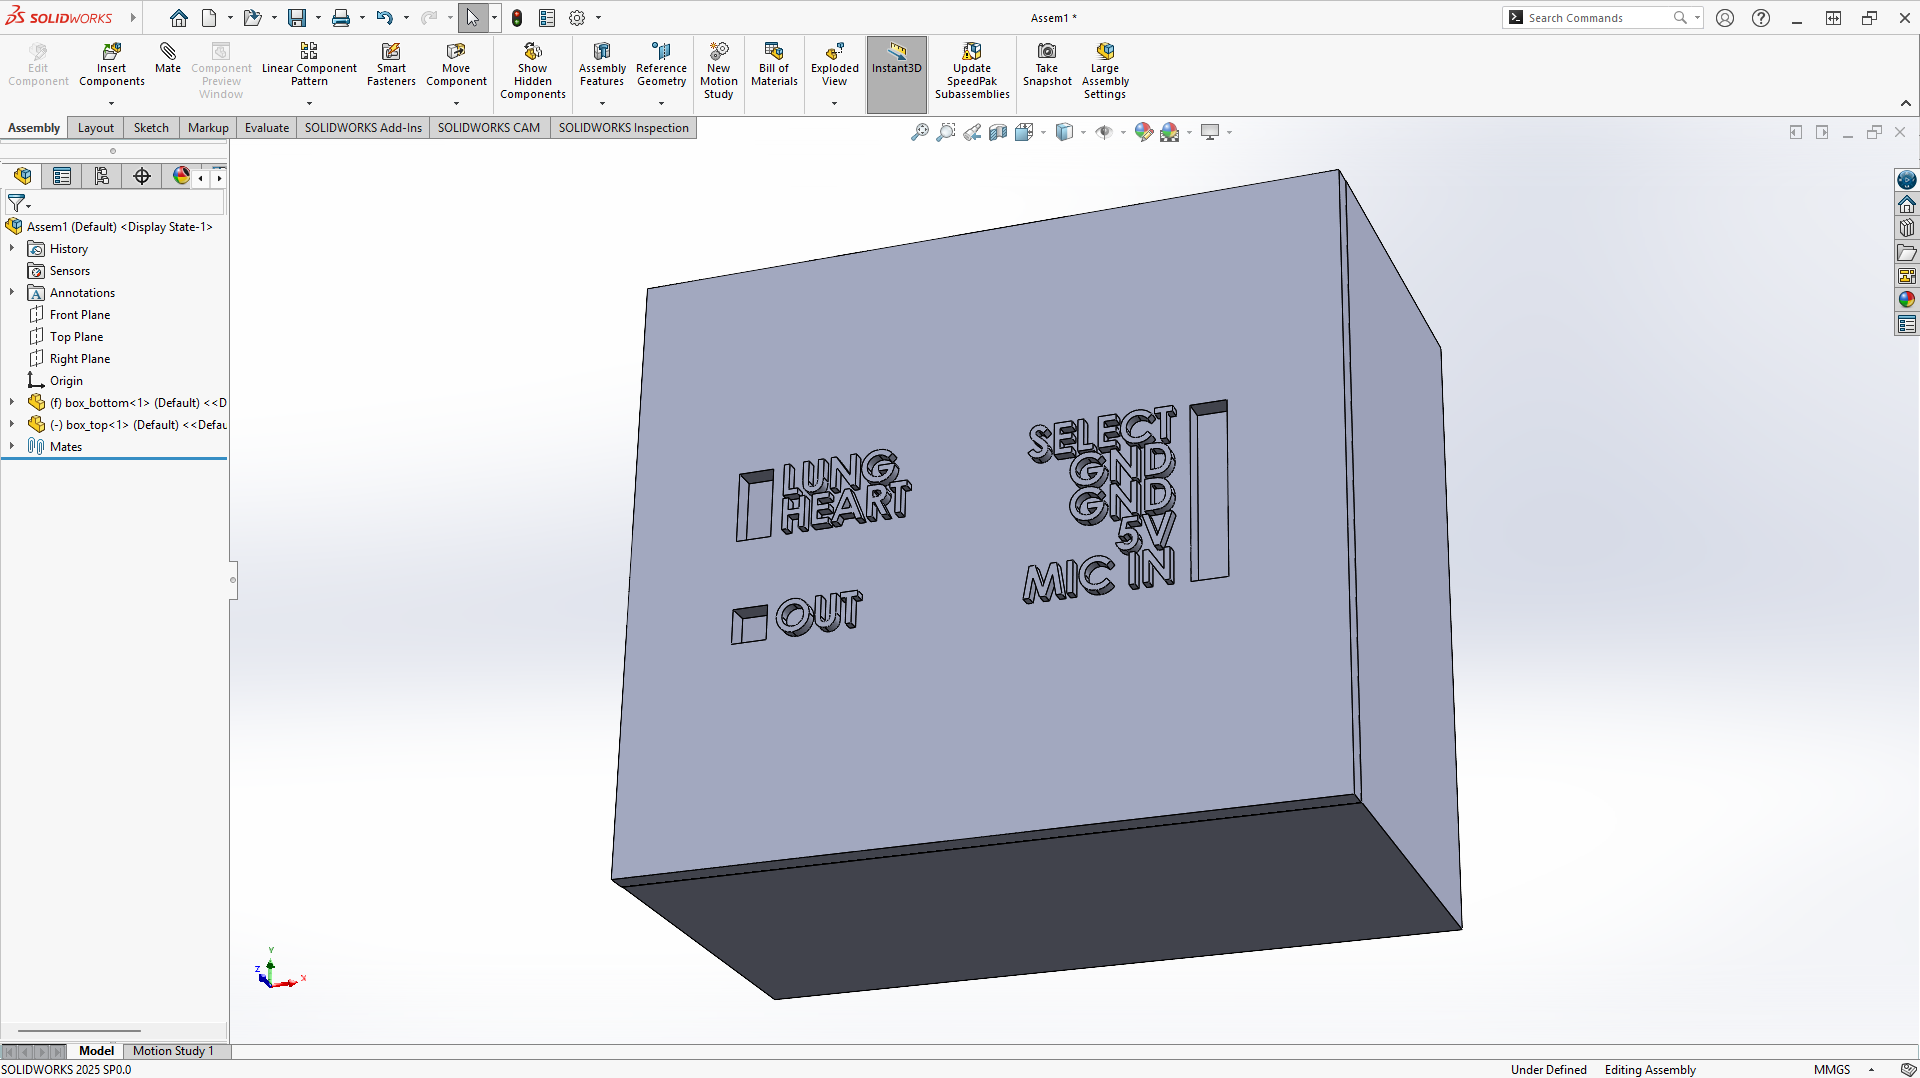
\includegraphics[width=0.7\textwidth]{assets/3d-design.png}
	\caption{Casing Design}
	\label{fig:casing_design}
\end{figure}

\begin{figure}[h]
	\centering
	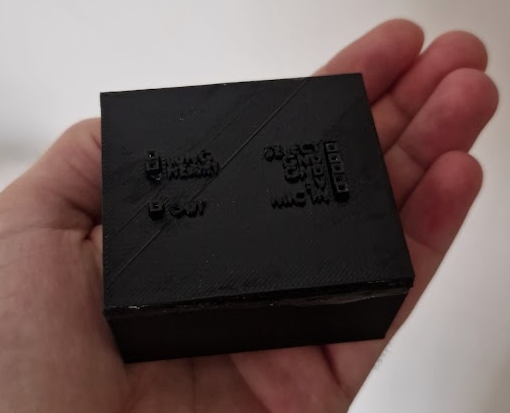
\includegraphics[width=0.5\textwidth]{assets/3d-design-printed.png}
	\caption{Casing Design Printed}
	\label{fig:casing_design_printed}
\end{figure}

Our first prototype is worked as expected so we decided to use it as our final prototype. By putting the prototype in the casing, we completed the hardware development phase.
